%=========================================================================
% (c) 2011, 2012 Josef Lusticky <xlusti00@stud.fit.vutbr.cz>

\section{Network}\label{sec:ntp-network}
Network specification of NTP defines that
the protocol uses the User Datagram Protocol (UDP) on port number 123~\cite{ianna-ports,rfc5905}.
Reliable message delivery such as TCP can actually make the delivered NTP packet less reliable since retries
would increase the delay value and other errors~\cite{rfc5905}.
This is mostly due to overhead of communication with TCP on transport layer.

All NTP time values are represented in twos-complement format, with
bits numbered in big-endian fashion from zero starting at the left, or high-order, position~\cite{rfc5905}. 
There are two formats of timestamp in NTP packet structure:
long 64-bit and short 32-bit as shown on figure~\ref{fig:ntp-timestamps}.
The 64-bit long timestamp used by NTP consists of a 32-bit unsigned seconds
field spanning 136 years (from 1900 to 2036) and a 32-bit fraction field resolving 232
picoseconds~\cite{rfc5905}.

%\!!
%An NTP timestamp is a truncated NTP date expressed as
%an unsigned 64-bit integer including the low order 32 bits of
%the seconds field concatenated with the high-order 32 bits of
%the fraction field.
%This format can represent the 136 years from 1900 to 2036 with a precision of 232 ps.
%\!!

The short 32-bit timestamp includes a 16-bit unsigned seconds field
and 16-bit fraction field.
Root dispersion is accumulated total dispersion from primary server.

\begin{figure}
	\centering
	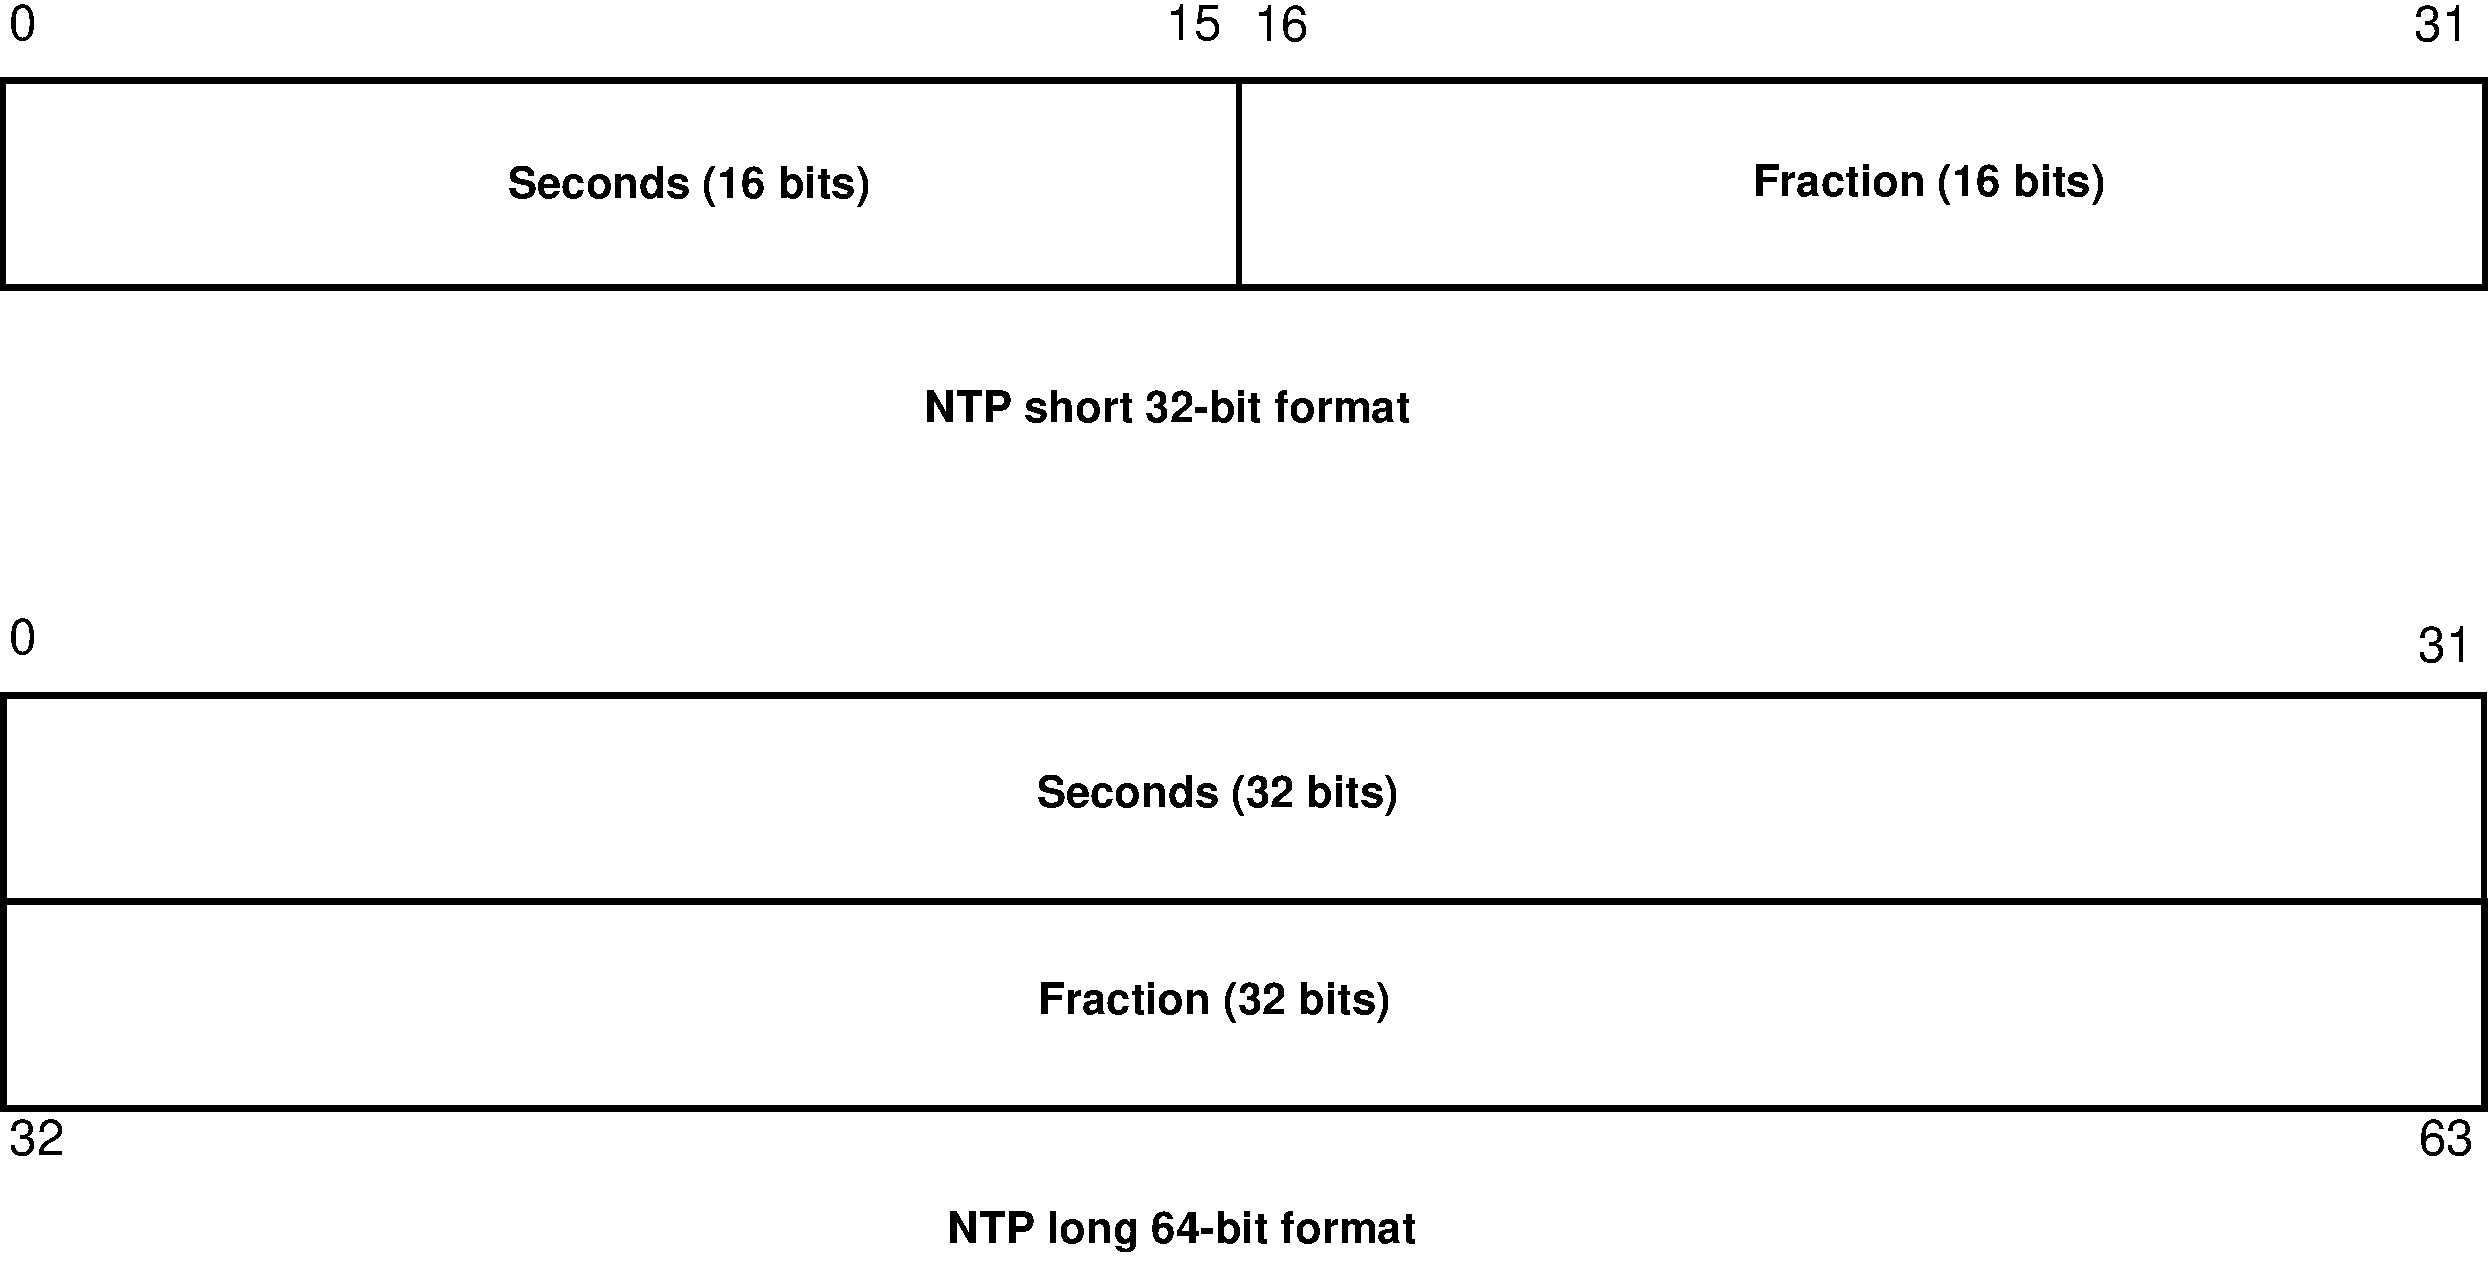
\includegraphics[width=13cm,keepaspectratio]{fig/ntp-timestamps.pdf}
	\caption{Formats used in NTP}
	\label{fig:ntp-timestamps}
	\bigskip
\end{figure}

% TODO - packet

\begin{figure}
	\centering
	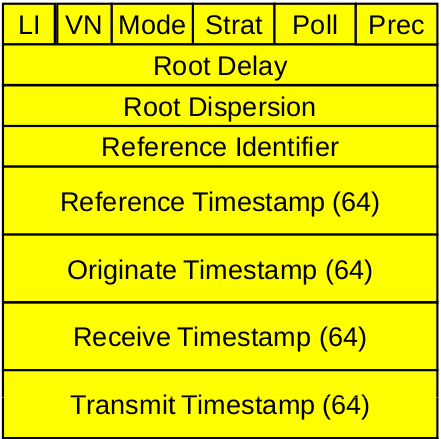
\includegraphics[width=6cm,keepaspectratio]{fig/ntp-packet.png}
	\caption{Basic NTP packet structure}
	\label{fig:ntp-packet}
	\bigskip
\end{figure}


Because the short 32-bit format is used for Root dispersion and Root Delay fields,
they do not need so big scope and precision.
Root dispersion express accumulated total dispersion from primary server
and Root Delay express accumulated roundtrip delay via primary server~\cite{ntp-arch}.

%TODO

Because of network latency the timestamp recieved will never be exactly corresponding to
the current time.
One of the main goals of NTP is to deal with the network latency~\cite{ntp-overview}.

